\section{A faster graph search can preserve the wrong relationship}
\label{repair29:discovery}

Before a bank asks whether a higher deposit rate attracts balances, it must
distinguish the effect of changing the rate from the information that led it
to offer that rate. A graph search can help compare explanations, but its
computational shortcuts have scientific consequences. A link retained because
the search stopped is a different finding from a relationship that survived
the relevant tests.

The detailed Java comparison in Section~\ref{why-conditioning-on-every-neighbour-is-not-a-safe-shortcut} identifies a concrete difficulty in the
inspected Aitiotita revision. Beyond conditioning depth two, one skeleton-search
path tests a pair conditional on the union of its neighbours. If dependence
persists, it marks the link undeletable and omits subsequent subset searches.
That rule would be safe only if dependence after adding variables excluded
independence under a smaller conditioning set. The retained generic callback
allows independence procedures for which that implication fails.
\citep{repair29pc}

This study examines a repair: continue the declared subset search, and
report an unfinished search explicitly when its budget is exhausted. The
calculations compare project implementations with exact independence oracles.
They do not execute the Java distribution. The distinction matters because
the inspected bundled linguistic oracle is not a Gaussian test, and the
orientation and graph-export stages require separate evaluation.

\subsection{A common consequence can undo a valid comparison}

Consider a hypothetical one-period decision. Let $X$ be a rate concession,
$Y$ a subsequent balance response and $Z_1,Z_2,Z_3$ three measured factors
known before the decision. The variables are centred model units; their
coefficients are stipulated, not bank estimates. Each baseline factor affects
both the offered rate and the balance. After the outcome, a score $C$ summarises
the concession and balance response. It is a common consequence, rather than
an additional baseline cause.

\begin{figure}[htbp]
\centering
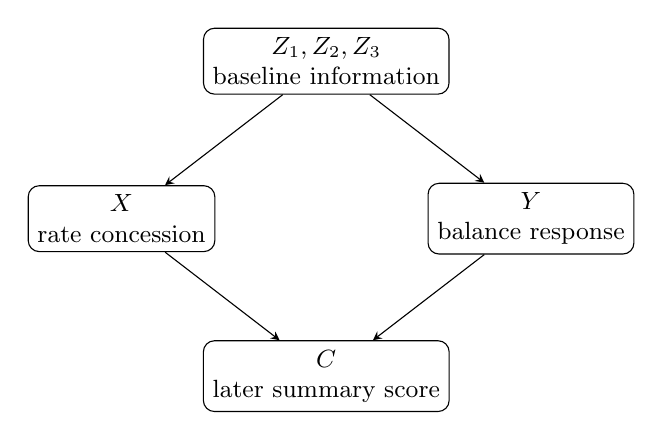
\begin{tikzpicture}[>=stealth, every node/.style={font=\small}]
\node[draw,rounded corners,align=center] (z) at (0,2) {$Z_1,Z_2,Z_3$\\baseline information};
\node[draw,rounded corners,align=center] (x) at (-2.6,0) {$X$\\rate concession};
\node[draw,rounded corners,align=center] (y) at (2.6,0) {$Y$\\balance response};
\node[draw,rounded corners,align=center] (c) at (0,-2) {$C$\\later summary score};
\draw[->] (z)--(x);\draw[->] (z)--(y);
\draw[->] (x)--(c);\draw[->] (y)--(c);
\end{tikzpicture}
\caption{Each baseline factor points to both $X$ and $Y$; the box groups the
three factors for readability. There is no causal arrow from $X$ to $Y$ in
this constructed example. Conditioning on their later common consequence
$C$ nevertheless makes their residuals associated.}
\label{repair29:collider}
\end{figure}

Let all six inputs $Z_1,Z_2,Z_3,\varepsilon_X,\varepsilon_Y,\varepsilon_C$
be mutually independent standard normal variables. The structural equations
are
\begin{align}
X&=Z_1+Z_2+Z_3+\varepsilon_X,\\
Y&=Z_1+Z_2+Z_3+\varepsilon_Y,\\
C&=X+Y+\varepsilon_C.
\end{align}
An intervention replacing the first equation changes $X$ and then $C$.
It leaves the equation for $Y$ unchanged. The mean effect on $Y$ is therefore
zero. In contrast, the unadjusted regression coefficient of $Y$ on $X$ is
$\operatorname{Cov}(X,Y)/\operatorname{Var}(X)=3/4$: common causes produce a
positive association without a treatment effect.

After adjusting for the three baseline factors, the residuals are
$X^*=\varepsilon_X$, $Y^*=\varepsilon_Y$ and
$C^*=\varepsilon_X+\varepsilon_Y+\varepsilon_C$. Thus
$\operatorname{Cov}(X^*,Y^*)=0$, and Gaussianity makes this conditional
independence. Adding the later score to the adjustment gives instead
\begin{align}
\operatorname{Cov}(X,Y\mid Z_1,Z_2,Z_3,C)
 &=0-\frac{\operatorname{Cov}(X^*,C^*)
                 \operatorname{Cov}(C^*,Y^*)}{\operatorname{Var}(C^*)}
 =-\frac13,\\
\operatorname{Var}(X\mid Z_1,Z_2,Z_3,C)&=1-\frac13=\frac23.
\end{align}
The corresponding regression coefficient is $(-1/3)/(2/3)=-1/2$.
Among customers with the same later score, a larger concession must tend
to accompany a smaller balance residual. This restriction is created by the
comparison, not by the intervention. The same structural law therefore has
a true effect of zero, an unadjusted slope of $3/4$, a baseline-adjusted slope
of zero and an overadjusted slope of $-1/2$.

Exact rational arithmetic verifies that none of the eleven conditioning sets
of size at most two separates $X$ and $Y$. At depth three the baseline set
does separate them, but the union of their neighbours also contains $C$.
The all-neighbour screen sees the nonzero conditional covariance and prevents
the valid subset from being tested. Four- and five-common-cause versions
produce the same $-1/2$ overadjusted slope, while their unadjusted slopes are
$4/5$ and $5/6$. The counterexample is consequently not peculiar to a single
three-factor covariance matrix.

For a bank, the immediate remedy is to respect the information clock and
preserve the distinction between adjustment candidates and later outcomes.
Removing the later score from the baseline information is economically
justified here. A general-purpose search still needs to handle colliders
correctly when they belong to its stated graph. The calculation does not
justify deleting inconvenient variables until a desired answer appears.

\subsection{Compare the repaired search on the same questions}

Both project searches start from the same complete undirected graph. At
each depth they test the same distinct subsets from each endpoint's
neighbourhood and remove separated pairs at the end of the depth. One search
adds the inspected screening rule; the repaired search does not. Freezing
neighbourhoods within a depth makes the comparison insensitive to the order
in which links are removed during that depth. Identical subsets available
from both endpoints are counted once in both implementations.

The principal oracle constructs the ancestral graph of the queried pair
and conditioning set, joins parents of each included node, and checks
connectivity after deleting conditioned nodes. An independently written
oracle enumerates paths and checks whether each internal node blocks or
opens the path. They agree on all conditioning queries for every ordered
four-variable graph and all queries used in the constructed witness family:
3,090 comparisons in total. The generating graph supplies the separate
reference skeleton. These checks address errors in the experiment itself;
they are not a theorem about every graph or a calibration study for noisy data.

\begin{table}[htbp]
\centering\small
\begin{tabular}{lrrrr}
\toprule
Declared case group & Cases & Full errors & Screen errors & Depth-2 errors\\
\midrule
All ordered graphs, 2--5 variables & 1,098 & 0 & 0 & 66\\
Seeded six-variable graphs & 256 & 0 & 22 & 72\\
Common-cause witness family & 3 & 0 & 3 & 3\\
Relabelled six-variable witness & 24 & 0 & 24 & 24\\
\bottomrule
\end{tabular}
\caption{An error means the returned undirected skeleton differs from the
generating skeleton. Every query uses an exact population independence
oracle. The seeded graphs use four declared edge probabilities; these
frequencies are descriptive of this finite suite, not estimates of failures
among banking applications. Relabellings are checks of the same witness,
not independent scientific replications.}
\label{repair29:results}
\end{table}

The full search recovers the reference skeleton on all 1,381 declared cases.
The screened search fails on 49, including 22 of the 256 seeded six-variable
graphs and all witness cases. Its success on every graph with at most five
variables would therefore give false reassurance if small examples alone
were used to judge it. The repair removes the observed logical obstruction
within the tested scope. It supplies no evidence that a selected finite-sample
test is sufficiently accurate, or that the data are faithful to a causal graph.

Counting independence requests reveals the cost of the shortcut. On the
ordered two-to-five-variable group, screening makes 46,856 requests versus
43,090 for full search: the extra screening step costs more than it saves.
On the seeded six-variable group it makes 25,651 requests versus 29,483,
but returns 22 wrong skeletons. These are calls in matched project searches,
not measurements of elapsed time in the Java product. An implementation
choice should compare accuracy and cost on the same declared task rather
than treat fewer calls as a scientific improvement.

\subsection{A computation budget should leave an honest question open}

A depth limit can be sensible when there are many variables. It changes
what has been learned. In the depth-two comparison, 165 cases return a
skeleton different from the generating one. Each of those cases is explicitly
marked incomplete because larger neighbouring conditioning sets remain
untested. The same warning also appears in some cases whose returned
skeleton happens to be correct. A stopping rule cannot know that fortunate
outcome without doing the omitted work or imposing additional justified
restrictions.

For the hypothetical bank, a retained $X$--$Y$ link is therefore insufficient
grounds to value a repricing policy. A report should distinguish the
independences actually found, the remaining candidate links, and the
search that was left unfinished. A graph skeleton alone also leaves arrow
directions and intervention effects unresolved. The economic next step may
be stronger pre-decision measurement, a justified model restriction or an
experiment; another graph-search heuristic need not supply the missing fact.

The proposal recommendation is to retain full subset search as the declared
reference and exclude this all-neighbour freezing rule for a general
Gaussian-oracle adaptation. A bounded implementation should return an
incomplete-search result when it stops early. Native package comparisons,
sampling calibration, orientation, prior-knowledge enforcement and endpoint
preservation remain distinct prototype tests. This result closes a specific
repair question and sharpens the software selection; it does not close the
complete Java survey or establish a bank-ready discovery engine. The following sampling comparison addresses one of these separate questions.

\section{A complete search can still give an incomplete lending comparison}
\label{closure30:sampling}

A bank can remove an unsound computational shortcut and still obtain an
unreliable effect estimate. The preceding exact-oracle comparison establishes
what the search does when every independence answer is correct. Actual records
offer estimates of those answers. A relationship that is weak after adjustment
may disappear from an estimated graph even when its economic contribution is
substantial. If that disappearance then removes a confounder from a lending
comparison, a narrow confidence interval can surround the wrong quantity.

This distinction motivates a second, deliberately limited study. It asks how
sampling error in the repaired search can affect the controls used to compare
rate concessions and balance responses. It also asks whether the bank's
information clock helps: should a score produced after the balance response
enter the discovery exercise in the first place? The examples are constructed
Gaussian economies with known equations. Their role is to expose a failure
mechanism and evaluate one response, not to estimate its prevalence in banks.

\subsection{An independence test is not a confidence statement about the graph}

For centred Gaussian variables, conditional independence between $X_i$ and
$X_j$ given $X_S$ is equivalent to a zero partial correlation
$\rho_{ij\mid S}$. The sample test used here follows the Fisher transformation
in \citet[Section 2.2.2, equation (3)]{kalisch2007}:
\begin{equation}
 Z_{ij\mid S}=\frac12\log\frac{1+\widehat\rho_{ij\mid S}}
                                  {1-\widehat\rho_{ij\mid S}},\qquad
 T_{ij\mid S}=\sqrt{n-|S|-3}\,|Z_{ij\mid S}|.
 \label{closure30:fisher}
\end{equation}
The search treats the pair as independent when
$T_{ij\mid S}\leq\Phi^{-1}(1-\alpha/2)$, where $n$ is the number of
observations, $|S|$ is the number of conditioning variables and $\Phi$ is the
standard normal distribution function. Failure to reject a zero correlation
is operationally used to delete the candidate link. It is not proof that the
population correlation is zero.

The same source's consistency result requires more than a large sample. Its
assumptions include a faithful Gaussian law, graph sparsity and bounds on
nonzero partial correlations; the asymptotic significance sequence depends on
an unknown lower signal bound. These conditions do not supply a finite-sample
guarantee at a fixed threshold. \citep[Assumptions A1--A4 and Theorem 1,
pp.~619--620]{kalisch2007}

The stable search stores each variable's neighbours at the beginning of a
conditioning depth, so deleting one link does not change the other candidate
sets examined at that depth. This is the central skeleton modification in
\citet[Section 4.1, Algorithm 4.1 and Theorem 3]{exec13_latentr_colombo2014}. It removes
one source of dependence on variable order. It does not make a noisy test
correct. The project comparison retains this level-frozen search and evaluates
all distinct candidate sets, rather than claiming a byte-for-byte reproduction
of a released software package.

For a small nonzero $\rho$, the approximate signal is
\[
 \sqrt{n-|S|-3}|\operatorname{atanh}(\rho)|.
\]
At a five per cent two-sided threshold, equating that scale to 1.96 gives
\begin{equation}
 n\approx |S|+3+
 \left\{\frac{1.96}{|\operatorname{atanh}(\rho)|}\right\}^{2}.
 \label{closure30:signal-scale}
\end{equation}
This is a signal-to-threshold calculation, not a power formula or a sample-size
recommendation. A correlation of about 0.00433 makes its last term approximately
205,000; a correlation of about 0.0289 makes it about 4,595. Large coefficients
elsewhere in a system do not ensure that every conditional comparison has a
large signal.

\subsection{Three economies with known intervention effects}

Let $Z=(Z_1,Z_2,Z_3)^\top$ denote independent baseline characteristics,
$X$ a rate concession and $Y$ the subsequent balance response. Let $C$ be a
later summary. The first two mechanisms are
\begin{align}
 X&=s\left(Z_1+\frac45Z_2+\frac65Z_3\right)+\varepsilon_X,\\
 Y&=s\left(\frac7{10}Z_1+\frac{11}{10}Z_2+
                 \frac9{10}Z_3\right)+\varepsilon_Y,\\
 C&=\frac{11}{10}X+\frac35Y+\varepsilon_C,
 \label{closure30:sampling-economy}
\end{align}
where the six exogenous inputs are mutually independent standard normal
variables. The larger-coefficient case has $s=1$; the smaller-coefficient case
has $s=1/8$. These are standardized model units. Neither coefficient choice is
an estimate for an institution. Changing $X$ leaves the structural equation
for $Y$ unchanged, so the intervention effect is zero in both cases.

The unadjusted population slope is
\begin{equation}
 \frac{\operatorname{Cov}(X,Y)}{\operatorname{Var}(X)}
 =\frac{(133/50)s^2}{1+(77/25)s^2}.
 \label{closure30:omitted-slope}
\end{equation}
It equals $133/204\simeq0.652$ when $s=1$ and
$133/3354\simeq0.0397$ when $s=1/8$. Correct adjustment for all three baseline
variables makes the slope zero. Including $C$ after that adjustment introduces
a different error. The residuals satisfy
$C^*=(11/10)\varepsilon_X+(3/5)\varepsilon_Y+\varepsilon_C$, giving the
overadjusted slope
\begin{equation}
 -\frac{(11/10)(3/5)}{1+(3/5)^2}=-\frac{33}{68}\simeq-0.485.
 \label{closure30:later-slope}
\end{equation}
These population calculations explain the directions of the simulation errors.
They also show why extra precision cannot compensate for an invalid comparison.

Both six-variable distributions are faithful to their stipulated graphs:
exact rational conditional covariances agree with graph separation for every
pair and conditioning set, 240 queries per mechanism. Faithfulness nevertheless
allows very small nonzero correlations. In the larger-coefficient case,
$\rho_{Z_1,Y\mid Z_3,C}\simeq-0.00433$, although $Z_1$ directly enters the
equation for $Y$. The later score nearly cancels the remaining association.
The larger coefficients therefore do not imply uniform strength of every
discovery query.

The third mechanism makes the distinction exact rather than approximate:
\begin{equation}
 Z=\varepsilon_Z,\qquad X=Z+\varepsilon_X,\qquad
 Y=X-Z+\varepsilon_Y=\varepsilon_X+\varepsilon_Y.
 \label{closure30:cancellation}
\end{equation}
Its intervention effect is one, but $Z$ and $Y$ are marginally independent.
The direct and indirect contributions cancel. Its unadjusted slope is $1/2$,
while adjustment for $Z$ recovers one. This distribution is unfaithful to the
three-arrow graph. It is included as an explicit assumption failure, not as
evidence against a theorem that assumes faithfulness.

\subsection{What is compared on the same observations}

For each mechanism and each sample size $n\in\{100,500,2000\}$, the study
generates 200 independent samples. It applies thresholds $\alpha=0.01$ and
$0.05$ to three searches: full stable subsets, the all-neighbour dependence
screen and a depth-two cap. This gives 1,800 datasets and 10,800 search results.
The methods receive identical observations within each comparison. The depth
cap keeps its unfinished-search flag whenever relevant larger sets remain.

To reveal the consequence of graph errors, an explicitly naive rule chooses
baseline variables that are adjacent to both $X$ and $Y$ in the estimated
skeleton. It then regresses $Y$ on $X$ and those selected variables using the
same observations, reporting an ordinary 95 per cent Student-$t$ interval for
the coefficient on $X$. The later score $C$ is always excluded from this
regression by its information date. This rule is a diagnostic comparator;
common estimated neighbours are not asserted to be a valid general adjustment
criterion. The reference regression uses every stipulated baseline cause.

Coverage means the proportion of the 200 intervals that contain the known
intervention effect. It is distinct from graph recovery. A graph can be wrong
in an economically irrelevant edge while the selected adjustment is correct,
or it can lose exactly the variable needed to remove confounding. The study
does not isolate the pure penalty from reusing observations after selection:
its interval failures combine selection, omitted confounders and inappropriate
confidence in the resulting regression. Splitting the sample would not by
itself make an invalid adjustment set valid.

\begin{table}[htbp]
\centering\small
\begin{tabular}{lrrrrr}
\toprule
Mechanism & $n$ & Wrong graphs & Selected coverage & Baseline coverage & Bias\\
\midrule
Larger coefficients &100&200/200&0.0\%&93.0\%&0.650\\
 &500&200/200&0.0\%&94.0\%&0.644\\
 &2000&200/200&0.0\%&95.5\%&0.635\\
Smaller coefficients &100&200/200&93.0\%&95.5\%&0.032\\
 &500&200/200&86.0\%&93.0\%&0.034\\
 &2000&191/200&81.5\%&97.0\%&0.023\\
Exact cancellation &100&187/200&6.5\%&94.5\%&$-0.468$\\
 &500&188/200&6.0\%&95.5\%&$-0.470$\\
 &2000&189/200&5.5\%&93.5\%&$-0.471$\\
\bottomrule
\end{tabular}
\caption{Full stable search at $\alpha=0.05$. Wrong graphs compares the
undirected skeleton with the stipulated graph; the cancellation case violates
faithfulness. Selected coverage uses the naive estimated-common-neighbour
rule. Baseline coverage uses all stipulated baseline causes. Bias is the
mean selected estimate minus the true effect, in model units. These are
descriptive simulation results, not bank performance estimates.}
\label{closure30:sampling-results}
\end{table}

The smaller-coefficient case illustrates how more observations can expose
rather than remove a comparison error. The selected estimator's bias remains
positive while its intervals narrow. Coverage falls from 93 to 81.5 per cent.
For the latter proportion, a descriptive 95 per cent Wilson Monte Carlo
interval is 75.5--86.3 per cent. It quantifies variation over the declared
independent simulation draws; it is not an interval for performance across
unknown banking environments.

In the larger-coefficient case, the selected rule almost always omits important
causes. At $n=2000$ the full search selects no baseline variable in 145 of 200
samples and selects only $Z_3$ in another 54. No interval contains the zero
effect. The ordinary all-baseline regression covers zero in 191 of those same
200 samples. The failure is therefore consequential for the lending contrast,
not simply a disagreement over an incidental arrow.

The screen and depth cap do not solve this sampling problem. At $n=2000$ in
the larger-coefficient case, full search retains the spurious $X$--$Y$ link in
193 samples; the screened and capped searches retain it in all 200. The depth
cap labels every one of these searches unfinished. Full search has completed
its declared tests, but sampling error still prevents correct recovery.
Completion and correctness are separate statements.

The stricter threshold does not provide reassurance. At $\alpha=0.01$, full
search in the smaller-coefficient case with $n=2000$ has only 67.0 per cent
interval coverage, compared with 81.5 per cent at $\alpha=0.05$. A smaller
significance level makes it easier to fail to reject a zero partial correlation and
delete a true link. The complete comparison below retains both thresholds;
neither should be chosen retrospectively to make this example look favorable.

\subsection{The information clock helps, but does not guarantee recovery}

After inspecting those results, a separately specified follow-up changes one
thing: it excludes $C$ from the discovery exercise as well as from the outcome
regression. Coefficients, sample sizes, thresholds, seeds and observations are
unchanged. Removing this particular node does not conceal a common cause:
it is only a later descendant of $X$ and $Y$. The reduced five-variable
covariances are verified against the corresponding graph. The cancellation
case contains no such node and is not rerun.

For the smaller-coefficient case at $n=2000$ and $\alpha=0.05$, full-search
coverage rises from 81.5 to 97.0 per cent. The paired difference is 15.5
percentage points, with a Monte Carlo standard error of 2.66 points. The
reference set of all three causes is selected in 188 samples. Exact skeleton
recovery rises from nine out of 200 for the six-variable task to 173 out of
200 for the five-variable task. The graph tasks differ because the latter
omits $C$; retained paired records also compare the common five-variable edges.

The larger-coefficient case improves much less. At $n=2000$, interval coverage
is still only 3.5 per cent and the reduced skeleton is wrong in 194 samples.
Even after removing $C$, conditioning on other variables leaves some direct-edge
correlations close to zero. Correct timing is useful economic information; it
does not guarantee a favorable statistical signal or establish faithfulness.

\begin{figure}[htbp]
\centering
\includegraphics[width=.78\textwidth]{twelve-hour-closure/2026-10-29/sampling-figures/coverage.pdf}
\caption{Coverage of ordinary 95 per cent effect intervals under full search,
$\alpha=0.05$, and 200 samples per point. Error bars are descriptive 95 per cent
Wilson Monte Carlo intervals. The green reference uses all stipulated baseline
causes; the blue follow-up excludes the later score from discovery. The dashed
line marks nominal coverage. These examples demonstrate specific failure and
repair mechanisms, not a general ranking of discovery methods.}
\label{closure30:coverage-figure}
\end{figure}

\subsection{What the proposal should require before valuing a graph}

The study supports a conditional recommendation. Keep full subset search as a
logical reference and report unfinished searches honestly. Also retain the
economically defended information clock, assess the signals required by the
discovery procedure, and justify the adjustment used for the particular lending
contrast. A graph can help formulate questions without supplying a qualified
effect estimate. A significance setting such as 0.05 should never be presented
as a 95 per cent probability that the entire graph is correct.

The numerical checks target the study itself. Exact rational covariance and
independently implemented graph/path tests agree on every declared population
query in the faithful cases. Precision-matrix and residual-regression partial
correlations agree within $5\times10^{-15}$ in 486 sample checks. Independent
QR residualization reproduces 270 retained interval calculations within
$7\times10^{-16}$; reversing variable order preserves the checked full-search
skeletons. These checks reduce implementation error in the examples. They
cannot establish a universal calibration guarantee.

All 54 first-study method/threshold cells and all 36 timing-follow-up cells
are retained, including adverse results. The follow-up was specified after
the first study and is described as such. Neither experiment evaluates native
R or Java software, arrow orientation, latent confounding, a live language
model or an actual bank. Those questions retain their own tests. For the
proposal, the scientific advance is narrower and useful: repairing the search
does not complete the causal comparison, and timing information can change
its reliability without making it universally reliable.

\subsection{Complete method and threshold comparisons}

The following tables retain every declared comparison. Strong and weak denote
the larger- and smaller-coefficient mechanisms above; cancellation denotes
the explicitly unfaithful mechanism. Full, screen and depth2 mean full stable
subsets, the all-neighbour screen and the depth-two cap. Each row contains
200 samples. Wrong and unfinished are counts, whereas coverage is the
percentage of ordinary selected-regression intervals containing the stipulated
effect. Equal coverage can coexist with different graph errors when the
errors leave the selected baseline controls unchanged.

\begingroup\small
\begin{longtable}{llrrrrr}
\toprule
Mechanism & Search & $n$ & $\alpha$ & Wrong & Unfinished & Coverage\\
\midrule\endhead
cancellation & depth2 & 100 & 0.01 & 197 & 0 & 1.5\%\\
cancellation & full & 100 & 0.01 & 197 & 0 & 1.5\%\\
cancellation & screen & 100 & 0.01 & 197 & 0 & 1.5\%\\
cancellation & depth2 & 100 & 0.05 & 187 & 0 & 6.5\%\\
cancellation & full & 100 & 0.05 & 187 & 0 & 6.5\%\\
cancellation & screen & 100 & 0.05 & 187 & 0 & 6.5\%\\
cancellation & depth2 & 500 & 0.01 & 199 & 0 & 0.5\%\\
cancellation & full & 500 & 0.01 & 199 & 0 & 0.5\%\\
cancellation & screen & 500 & 0.01 & 199 & 0 & 0.5\%\\
cancellation & depth2 & 500 & 0.05 & 188 & 0 & 6.0\%\\
cancellation & full & 500 & 0.05 & 188 & 0 & 6.0\%\\
cancellation & screen & 500 & 0.05 & 188 & 0 & 6.0\%\\
cancellation & depth2 & 2000 & 0.01 & 195 & 0 & 2.5\%\\
cancellation & full & 2000 & 0.01 & 195 & 0 & 2.5\%\\
cancellation & screen & 2000 & 0.01 & 195 & 0 & 2.5\%\\
cancellation & depth2 & 2000 & 0.05 & 189 & 0 & 5.5\%\\
cancellation & full & 2000 & 0.05 & 189 & 0 & 5.5\%\\
cancellation & screen & 2000 & 0.05 & 189 & 0 & 5.5\%\\
strong & depth2 & 100 & 0.01 & 200 & 0 & 0.0\%\\
strong & full & 100 & 0.01 & 200 & 0 & 0.0\%\\
strong & screen & 100 & 0.01 & 200 & 0 & 0.0\%\\
strong & depth2 & 100 & 0.05 & 200 & 15 & 0.0\%\\
strong & full & 100 & 0.05 & 200 & 0 & 0.0\%\\
strong & screen & 100 & 0.05 & 200 & 0 & 0.0\%\\
strong & depth2 & 500 & 0.01 & 200 & 187 & 0.0\%\\
strong & full & 500 & 0.01 & 200 & 0 & 0.0\%\\
strong & screen & 500 & 0.01 & 200 & 0 & 0.0\%\\
strong & depth2 & 500 & 0.05 & 200 & 198 & 0.0\%\\
strong & full & 500 & 0.05 & 200 & 0 & 0.0\%\\
strong & screen & 500 & 0.05 & 200 & 0 & 0.0\%\\
strong & depth2 & 2000 & 0.01 & 200 & 200 & 0.0\%\\
strong & full & 2000 & 0.01 & 200 & 0 & 0.0\%\\
strong & screen & 2000 & 0.01 & 200 & 0 & 0.0\%\\
strong & depth2 & 2000 & 0.05 & 200 & 200 & 0.0\%\\
strong & full & 2000 & 0.05 & 200 & 0 & 0.0\%\\
strong & screen & 2000 & 0.05 & 200 & 0 & 0.0\%\\
weak & depth2 & 100 & 0.01 & 200 & 0 & 93.0\%\\
weak & full & 100 & 0.01 & 200 & 0 & 93.0\%\\
weak & screen & 100 & 0.01 & 200 & 0 & 93.0\%\\
weak & depth2 & 100 & 0.05 & 200 & 1 & 93.0\%\\
weak & full & 100 & 0.05 & 200 & 0 & 93.0\%\\
weak & screen & 100 & 0.05 & 200 & 0 & 93.0\%\\
weak & depth2 & 500 & 0.01 & 200 & 2 & 85.5\%\\
weak & full & 500 & 0.01 & 200 & 0 & 85.5\%\\
weak & screen & 500 & 0.01 & 200 & 0 & 85.5\%\\
weak & depth2 & 500 & 0.05 & 200 & 11 & 86.0\%\\
weak & full & 500 & 0.05 & 200 & 0 & 86.0\%\\
weak & screen & 500 & 0.05 & 200 & 0 & 86.0\%\\
weak & depth2 & 2000 & 0.01 & 200 & 29 & 67.0\%\\
weak & full & 2000 & 0.01 & 200 & 0 & 67.0\%\\
weak & screen & 2000 & 0.01 & 200 & 0 & 67.0\%\\
weak & depth2 & 2000 & 0.05 & 191 & 86 & 81.5\%\\
weak & full & 2000 & 0.05 & 191 & 0 & 81.5\%\\
weak & screen & 2000 & 0.05 & 191 & 0 & 81.5\%\\
\bottomrule\end{longtable}

\endgroup

The timing follow-up omits the later descendant from discovery. Its final
column is the paired change in coverage, in percentage points, relative to
the corresponding first-study row. The graph-error columns concern the reduced
five-variable task and therefore have a different graph target from the first
table. This follow-up was specified after the first study; the comparison
does not acquire a prospective status retrospectively.

\begingroup\small
\begin{longtable}{llrrrrrr}
\toprule
Mechanism & Search & $n$ & $\alpha$ & Wrong & Unfinished & Coverage & Change\\
\midrule\endhead
strong & depth2 & 100 & 0.01 & 200 & 1 & 0.0\% & +0.0\\
strong & full & 100 & 0.01 & 200 & 0 & 0.0\% & +0.0\\
strong & screen & 100 & 0.01 & 200 & 0 & 0.0\% & +0.0\\
strong & depth2 & 100 & 0.05 & 200 & 4 & 0.0\% & +0.0\\
strong & full & 100 & 0.05 & 200 & 0 & 0.0\% & +0.0\\
strong & screen & 100 & 0.05 & 200 & 0 & 0.0\% & +0.0\\
strong & depth2 & 500 & 0.01 & 200 & 3 & 0.0\% & +0.0\\
strong & full & 500 & 0.01 & 200 & 0 & 0.0\% & +0.0\\
strong & screen & 500 & 0.01 & 200 & 0 & 0.0\% & +0.0\\
strong & depth2 & 500 & 0.05 & 200 & 13 & 0.0\% & +0.0\\
strong & full & 500 & 0.05 & 200 & 0 & 0.0\% & +0.0\\
strong & screen & 500 & 0.05 & 200 & 0 & 0.0\% & +0.0\\
strong & depth2 & 2000 & 0.01 & 200 & 49 & 0.0\% & +0.0\\
strong & full & 2000 & 0.01 & 200 & 0 & 0.0\% & +0.0\\
strong & screen & 2000 & 0.01 & 200 & 0 & 0.0\% & +0.0\\
strong & depth2 & 2000 & 0.05 & 200 & 117 & 3.5\% & +3.5\\
strong & full & 2000 & 0.05 & 194 & 0 & 3.5\% & +3.5\\
strong & screen & 2000 & 0.05 & 194 & 0 & 3.5\% & +3.5\\
weak & depth2 & 100 & 0.01 & 200 & 0 & 93.0\% & +0.0\\
weak & full & 100 & 0.01 & 200 & 0 & 93.0\% & +0.0\\
weak & screen & 100 & 0.01 & 200 & 0 & 93.0\% & +0.0\\
weak & depth2 & 100 & 0.05 & 200 & 0 & 93.0\% & +0.0\\
weak & full & 100 & 0.05 & 200 & 0 & 93.0\% & +0.0\\
weak & screen & 100 & 0.05 & 200 & 0 & 93.0\% & +0.0\\
weak & depth2 & 500 & 0.01 & 200 & 0 & 90.0\% & +4.5\\
weak & full & 500 & 0.01 & 200 & 0 & 90.0\% & +4.5\\
weak & screen & 500 & 0.01 & 200 & 0 & 90.0\% & +4.5\\
weak & depth2 & 500 & 0.05 & 189 & 4 & 92.0\% & +6.0\\
weak & full & 500 & 0.05 & 189 & 0 & 92.0\% & +6.0\\
weak & screen & 500 & 0.05 & 189 & 0 & 92.0\% & +6.0\\
weak & depth2 & 2000 & 0.01 & 41 & 4 & 95.5\% & +28.5\\
weak & full & 2000 & 0.01 & 40 & 0 & 95.5\% & +28.5\\
weak & screen & 2000 & 0.01 & 40 & 0 & 95.5\% & +28.5\\
weak & depth2 & 2000 & 0.05 & 31 & 9 & 97.0\% & +15.5\\
weak & full & 2000 & 0.05 & 27 & 0 & 97.0\% & +15.5\\
weak & screen & 2000 & 0.05 & 27 & 0 & 97.0\% & +15.5\\
\bottomrule\end{longtable}
\endgroup

The next chapter asks a prior question for any such search: whether recorded
variables and customer identities faithfully represent the economic observations
whose relationships are being learned.

